% !TeX root=main.tex
\iffalse
% You can copy any following box you like to your code.
\newtcolorbox{boxA}{
	fontupper = \bf,
	boxrule = 1.5pt,
	colframe = black % frame color
}

\begin{boxA}
	\lr{The box area is made visible by the shadow instead of the border. The top line may be placed on the left (replace border-top with border-left).}
\end{boxA}

\newtcolorbox{boxM}{
	fontupper = \color{white},
	rounded corners,
	arc = 6pt,
	colback = main!80, 
	colframe = main, 
	boxrule = 0pt, 
	bottomrule = 4.5pt,
	enhanced,
	fuzzy shadow = {0pt}{-3pt}{-0.5pt}{0.5pt}{black!35}
}
\begin{boxM}
	\lr{I added a shadow to give it a more three-dimensional appearance. It's a little flashy, so it might be good to use it on the part you really want to stand out.}
\end{boxM}
\fi


\chapter{روش پیشنهادی برای تشخیص موضع بدون داده آموزشی}

\setlength\parindent{0pt}   % killing indentation for all the text
\setstretch{1.3}            % setting line spacing to 1.3
\setlength\columnsep{0.25in} % setting length of column separator
\pagestyle{empty}           % setting pagestyle to be empty


\definecolor{main}{HTML}{5989cf}    % setting main color to be used
\definecolor{sub}{HTML}{cde4ff}     % setting sub color to be used

\newtcolorbox{boxK}{
	sharpish corners, % better drop shadow
	boxrule = 0pt,
	toprule = 4.5pt, % top rule weight
	enhanced,
	fuzzy shadow = {0pt}{-2pt}{-0.5pt}{0.5pt}{black!35} % {xshift}{yshift}{offset}{step}{options} 
}

\definecolor{ao(english)}{rgb}{0.0, 0.5, 0.0}
\definecolor{vividauburn}{rgb}{0.58, 0.15, 0.14}
\thispagestyle{empty}


امروزه استفاده از مدل‌های زبانی بزرگ برای حل مسائل مختلف پردازش زبان طبیعی بسیار فراگیر شده است. با استفاده از این مدل‌ها می‌توان بدون داده آموزشی یا با داده آموزشی کم و با طراحی یک پرامپت مناسب
\LTRfootnote{Prompt Engineering}
 نتایج قابل قبولی به دست آورد. در این پژوهش، به منظور استفاده از مدل‌های زبانی بزرگ در مسئله تشخیص موضع، چهار پرامپت با رویکردهای متفاوت پیشنهاد شد. پرامپت‌ها به صورت سلسله مراتبی تعریف شدند. بدین معنا که هر پرامپت اطلاعات بیشتری نسبت به پرامپت قبلی به عنوان ورودی دریافت می‌کنند. در ادامه هر یک از رویکردهای پیشنهادی به تفصیل توضیح داده می‌شود.


\section{روش حل مسئله}
در این پژوهش 4 پرامپت در سطح‌های متفاوت تعریف شدند. در طراحی پرامپت از قواعد پیشنهاد شده توسط بزرگ‌ترین توسعه دهندگان مدل‌های زبانی بزرگ (همچون 
\lr{OpenAI}) استفاده کردیم
\LTRfootnote{\href{https://platform.openai.com/docs/guides/prompt-engineering/six-strategies-for-getting-better-results}{https://platform.openai.com/docs/guides/prompt-engineering/six-strategies-for-getting-better-results}}.
اصول استفاده شده در طراحی پرامپت عبارتند از:
\begin{enumerate}
	\item نوشتن درخواست به صورت ساده و واضح و دقیق: باید ورودی و خروجی و مسئله‌ای که مدل قصد حل کردن آن را دارد به صورت کاملا واضح و شفاف توضیح داده شود. هر چه قدر توضیحات دقیق‌تر و کامل‌تری در پرامپت  باشد، احتمال رسیدن به پاسخ صحیح بیشتر می‌شود. همچنین مشخص کردن دقیق خروجی درخواستی از مدل، باعث بهبود نتایج می‌شود. وجود چند مثال از حل مسئله (رویکرد
\lr{Few Shot}\cite{10.5555/3495724.3495883}) 
نیز می‌تواند ایده مناسبی برای بهره‌مندی بیشتر مدل از پرامپت ورودی باشد.

\item تقسیم کردن مسئله اصلی به چند زیر مسئله ساده‌تر: نرخ پاسخگویی اشتباه در مسائل پیچیده بسیار بالاست. بنابراین یک راه حل بهینه این است که مسئله اولیه، در قالب چند زیر مسئله ساده‌تر تعریف شود. در ادامه گام‌های حل هر مسئله به صورت شفاف توضیح داده‌ شود تا احتمال رسیدن به پاسخ مطلوب افزایش یابد (رویکرد
\lr{Chain of Thought}
از این قاعده استفاده می‌کند). در این صورت به مدل زمان لازم برای استنتاج داده می‌شود و پاسخ‌های قابل اعتمادتری تولید می‌شود.
\end{enumerate}

با توجه به اصول مطرح شده به عنوان راهنما برای طراحی پرامپت، چهار پرامپت در سطوح مختلف با رویکرد‌های متفاوت تعریف شدند. در ادامه به توضیح چهار پرامپت پیشنهادی این پژوهش پرداخته می‌شود.

\subsection{پرامپت
\lr{Zero Shot}
}
در این پرامپت ساده‌ترین روش در نظر گرفته شد. پرامپت متشکل از توضیح مسئله، وظیفه خواسته شده از مدل، ورودی‌های مسئله تشخیص موضع شامل موضوع
\LTRfootnote{Target}
و متن توییت و مشخص نمودن کلاس‌های خروجی می‌باشد. در نوشتن پرامپت توضیحات به صورت دقیق و ساده ارائه شدند. شکل
\ref{zeroshot-prompt}
قالب پیشنهادی را نشان می‌دهد. 

\begin{figure}[H]
	\small
	\begin{boxK}
		\raggedright
		\lr{{The following statements (tweet) are twitter posts about {target}    target. Each statement can support, oppose, or be neutral toward its associated {target} belief and Each statement has the reason for that stance.}}\\
		\lr{Now, classify the following statement as to whether support, oppose, and neutral toward the belief below being true, and give your explanation for the classification.}\\
		\lr{Target: \texttt{<target>}}\\
		\lr{Tweet: \texttt{<tweet?}}\\
		\lr{Stance : {{select 'Stance' ['support', 'oppose', 'neutral'] }}}\\
		\lr{Explanation: {{gen 'explanation'}}}
	\end{boxK}
	\caption{\label{zeroshot-prompt}الگو پرامپت \lr{Zero Shot}}
\end{figure}

\subsection{پرامپت
	\lr{Zero Shot + Chain of Thought}
}
این رویکرد، در ادامه پرامپت
\lr{Zero Shot}
پیشنهاد شده است. در این پرامپت توضیحات مربوط به نحوه حل مسئله گام به گام توضیح داده شده به طوری که مدل زمان لازم برای استدلال را داشته باشد. همچنین با تقسیم مسئله به زیر مسئله‌های ساده‌تر مدل برای دستیابی به پاسخ صحیح راهنمایی می‌شود. شکل
\ref{zeroshot-Cot-prompt}
قالب پیشنهادی را نشان می‌دهد. قسمت مربوط به 
\lr{Chain of Thought (CoT)}
با رنگ 
\textcolor{blue}{آبی}
 مشخص شده است.
\begin{figure}[H]
	\small
	\begin{boxK}
		\raggedright
		\lr{{The following statements (tweet) are twitter posts about {target}    target. Each statement can support, oppose, or be neutral toward its associated {target} belief and Each statement has the reason for that stance.}}\\
		\lr{Now, classify the following statement as to whether support, oppose, and neutral toward the belief below being true, and give your explanation for the classification.}\\
		\lr{\textcolor{blue}{let's think step by step.}}\\
		\lr{\textcolor{blue}{First, check if the author of the tweet has commented on climate change. Has he commented at all? Then check if the author supports that climate change is a concern and should be addressed. Or is the author's opinion that this matter does not require special attention?}}\\
		\lr{Target: $<target>$}\\
		\lr{Tweet: \texttt{$<tweet>$}}\\
		\lr{Stance : {{select 'Stance' ['support', 'oppose', 'neutral'] }}}\\
		\lr{Explanation: {{gen 'explanation'}}}
	\end{boxK}
	\caption{\label{zeroshot-Cot-prompt}الگو پرامپت \lr{Zero Shot + Chain of Thought}}
\end{figure}


\subsection{پرامپت
\lr{Zero Shot + Chain of Thought + Context Description}
}

این پرامپت، در ادامه پرامپت
\lr{Zero Shot + Chain of Thought}
پیشنهاد شد. نقطه ضعف پرامپت‌های قبلی عدم وجود توضیحاتی راجع به موضوع تغییرات اقلیمی است و تنها تعریف مسئله تشخیص موضع در متن پرامپت وجود دارد. در این پرامت سعی شده توضیحاتی راجع به موضوع مورد بحث نیز به عنوان ورودی در نظر گرفته شود. توضیحات برگرفته از صفحه ویکی‌پدیا مربوطه می‌باشد. شکل
\ref{zeroshot-Cot-Context Description-prompt}
قالب پیشنهادی را نشان می‌دهد. قسمت مربوط به 
\lr{Context}
با رنگ
\textcolor{ao(english)}{سبز}
 مشخص شده است.
\begin{figure}[H]
	\small
	\begin{boxK}
		
		\raggedright
		\lr{The following statements (tweet) are twitter posts about Climate Change.	\textcolor{ao(english)}{Climate change describes global warming—the ongoing increase in global average temperature—and its effects on Earth's climate system. Climate change in a broader sense also includes previous long-term changes to Earth's climate.  Fossil fuel use, deforestation, and some agricultural and industrial practices add to greenhouse gases, notably carbon dioxide and methane. Greenhouse gases absorb some of the heat that the Earth radiates after it warms from sunlight.}
		 Each statement can support, oppose, or be neutral toward its associated {target} belief and Each statement has the reason for that stance.}\\
		\lr{Now, classify the following statement as to whether support, oppose, and neutral toward the belief below being true, and give your explanation for the classification.}\\
		\lr{\textcolor{blue}{let's think step by step.}}\\
		\lr{\textcolor{blue}{First, check if the author of the tweet has commented on climate change. Has he commented at all? Then check if the author supports that climate change is a concern and should be addressed. Or is the author's opinion that this matter does not require special attention?}}\\
		\lr{Target: \texttt{$<target>$}}\\
		\lr{Tweet: \texttt{$<tweet>$}}\\
		\lr{Stance : {{select 'Stance' ['support', 'oppose', 'neutral'] }}}\\
		\lr{Explanation: {{gen 'explanation'}}}
	\end{boxK}
	\caption{\label{zeroshot-Cot-Context Description-prompt}الگو پرامپت \lr{Zero Shot + Chain of Thought + Context Description}}
	
\end{figure}
\subsection{پرامپت
	\lr{Few Shot + Chain of Thought + Context Description}
}
تا این مرحله اطلاعات مناسبی به متن پرامپت ورودی اضافه شد. پرامپت پیشنهاد شده در این مرحله از رویکرد
	\lr{Few Shot + Chain of Thought + Context Description}
	پیروی می‌کند. در این پرامپت علاوه بر ورودی‌های قبلی، چند مثال از متن توییت و موضع توییت آورده شده است. در این روش سعی شده با دیدن چند نمونه آموزشی، بهبودی در عملکرد مدل ایجاد کنیم. شکل
	\ref{fewshot-Cot-Context Description-prompt}
	قالب پیشنهادی را نشان می‌دهد. نمونه‌های آموزشی در این پرامپت به صورت تصادفی انتخاب شدند. قسمت مربوط به 
	\lr{Few Shot}
	با رنگ
 \textcolor{vividauburn}{قهوه‌ای}
	  مشخص شده است.


\begin{figure}[H]
	\scriptsize
	\begin{boxK}
		\raggedright
		\lr{The following statements (tweet) are twitter posts about Climate Change.	\textcolor{ao(english)}{Climate change describes global warming—the ongoing increase in global average temperature—and its effects on Earth's climate system. Climate change in a broader sense also includes previous long-term changes to Earth's climate.  Fossil fuel use, deforestation, and some agricultural and industrial practices add to greenhouse gases, notably carbon dioxide and methane. Greenhouse gases absorb some of the heat that the Earth radiates after it warms from sunlight.} Each statement can support, oppose, or be neutral toward its associated {target} belief and Each statement has the reason for that stance.}\\
		\lr{\textcolor{vividauburn}{Let's see some example.}}\\
		\lr{\textcolor{vividauburn}{the tweet \texttt{$<tweet>$} stance on Climate change is supportive.}}\\
		\lr{\textcolor{vividauburn}{the tweet \texttt{$<tweet>$} stance on Climate change is opposite.}}\\
		\lr{\textcolor{vividauburn}{the tweet \texttt{$<tweet>$} stance on Climate change is neutral.}}\\
		\lr{Now, classify the following statement as to whether support, oppose, and neutral toward the belief below being true, and give your explanation for the classification.}\\
		\lr{\textcolor{blue}{let's think step by step}}\\
		\lr{\textcolor{blue}{First, check if the author of the tweet has commented on climate change. Has he commented at all? Then check if the author supports that climate change is a concern and should be addressed. Or is the author's opinion that this matter does not require special attention?}}\\
		\lr{Target: \texttt{$<target>$}}\\
		\lr{Tweet: \texttt{$<tweet>$}}\\
		\lr{Stance : {{select 'Stance' ['support', 'oppose', 'neutral'] }}}\\
		\lr{Explanation: {{gen 'explanation'}}}
	\end{boxK}
	\caption{\label{fewshot-Cot-Context Description-prompt}الگو پرامپت \lr{Few Shot + Chain of Thought + Context Description}}
\end{figure}

\section{آزمایش‌ها و تحلیل نتایج}
برای انجام آزمایش‌ها از مجموعه داده
\lr{ClimaConvo}\cite{shiwakoti2024analyzing}
و
\lr{SemEval}\cite{mohammad-etal-2016-semeval}
و مدل
\lr{Orca}\cite{orca-mini-v3-7b}
استفاده شد. به دلیل عملکرد مناسب مدل 
\lr{Orca}
در مقایسه با سایر مدل‌هایی با تعداد پارامتر مشابه از این مدل برای اجرا آزمایش‌ها استفاده شد (با توجه به سخت‌افزار موجود امکان استفاده از مدل‌های زبانی با پارامترهای بیشتر میسر نیست). در اجرا آزمایش‌ها پارامتر دما
\LTRfootnote{Temperature}
برابر با صفر قرار گرفت تا همواره توکن با بیشترین احتمال را تولید کند. از آن‌جایی که نتایج مدل‌های
\lr{Zero Shot}
برای مجموعه داده 
\lr{SemEval}
موجود بود، ابتدا مقایسه‌ای از روش‌های موجود شامل تکنیک‌های یادگیری عمیق و پرامپت با روش معرفی شده انجام شد. در جدول
~\ref{prompt-result-semeval}
پرامپت‌های پیشنهادی با سایر روش‌های یادگیری عمیق با رویکرد یادگیری بدون داده آموزشی مورد مقایسه قرار گرفت. نتایج به دست آمده نشان می‌دهد، در موضوع "قانونی شدن سقط جنین (\lr{LA})" پرامپت
\lr{Zero Shot}
از سایر روش‌های قبلی به صورت معناداری بهتر است. با توجه به نوع متن ورودی پرامپت، تنها رویکرد
\lr{Zero Shot}
برای این موضوع قابل استفاده بود. در موضوع " تغییرات اقلیمی (\lr{CC})" پرامپت 
\lr{Zero Shot + CoT}
عملکرد بهتری از خود نشان داده است و نسبت به نتایج
\lr{Bicond}
و 
\lr{GPT3.5}
به صورت معنادار بهتر است اما نسبت به سایرین عملکرد ضعیف‌تری دارد. به طور کلی قسمت
\lr{CC}
در مجموعه داده
\lr{SemEval}
در مقایسه با 
\lr{LA}
در اکثر مدل‌ها نتایج ضعیفی از خود نشان داده است. این نتایج نشان دهنده پیچیده‌تر بودن داده‌های این موضوع از مجموعه داده
\lr{SemEval}
می‌باشد.

\begin{table}[H]
	\centering
	\small
	\caption[مقایسه نتایج پرامپت‌های معرفی شده با سایر مدل‌های 
	\lr{Zero-Shot}]{\label{prompt-result-semeval}مقایسه نتایج 
		بر اساس معیار
		\lr{F1-Score}
		برای پرامپت‌های معرفی شده با سایر مدل‌های 
		\lr{Zero-Shot}
		بر مجموعه داده
		\lr{ SemEval}.}
	\vspace{0.2cm}
	\begin{tabular}{c  |c   c}
		\hline
		رویکرد & $LA$ & $CC$\\
		\hline
		\lr{Bicond} \cite{augenstein-etal-2016-stance} & $34.4$ & $15.0$\\
		\lr{CrossNet} \cite{xu-etal-2018-cross} & $34.4$ & -\\
		\lr{SEKT} \cite{zhang-etal-2020-enhancing-cross} & $44.6$ & -\\
		\lr{TPDG}  \cite{10.1145/3442381.3449790} &$46.5$ & -\\
		\lr{Bert\_Spc} \cite{devlin-etal-2019-bert}& $44.8$ & $37.3$\\
		\lr{Bert-GCN}  \cite{lin-etal-2021-bertgcn}& $44.2$& $35.5$\\
		\lr{PT-HCL}  \cite{10.1145/3485447.3511994}& $50.9$ & $38.9$\\
		\lr{GPT-3.5} \cite{zhang2022would} & $52.0$ & $24.7$\\
		\lr{GPT-3.5+COT} & $55.3$ & $25.2$\\
		%		\lr{ChatGPT} & $59.3$ &- \\
		\hline
		%sem eval P1: accuracy 0.3136094674556213	precision  0.3819444444444444		recall  0.2468517931932566	f1  0.23650540492645758
		
		پرامپت
		\lr{Zero Shot}  & \underline{$57.33 \dagger$}&  $23.65$ 
		\\
		پرامپت	
		%accuracy 0.40828402366863903		precision  0.4077519379844961		recall  0.2694330060183719		f1  0.28803700456510567
		\lr{Zero Shot + CoT}   & - & \underline{$28.80 \dagger$ }
		\\ 
		پرامپت
		%accuracy 0.25443786982248523	precision  0.36816578483245155	recall  0.15775173336148948 f1  0.19301094670997235
		
		\lr{Zero Shot + CoT + Context} & - & $19.30$ 
		\\
		پرامپت
		\lr{Few Shot + Cot + Context} & - & $20.85$ \\
		\hline
		\hline
	\end{tabular}
\end{table}



 در ادامه عملکرد پرامپت‌های معرفی شده بر روی مجموعه داده
 \lr{ClimaConvo}
 مورد بررسی قرار گرفت. هنگام انجام آزمایش‌های این قسمت، هیچ‌گونه پیش‌پردازشی در داده‌های متنی صورت نگرفته است. گزارش‌ها نشان می‌دهد 
 (جدول~
 \ref{prompt-result})
 همه نتایج به دست آمده نسبت به روش قبلی خود در سلسله مراتب به صورت معنی‌دار بهبود داشتند. همان‌طور که از نتایج مشخص است، پرامپت با رویکرد
 \lr{Few Shot}
 توانسته نتایج بسیار قابل قبولی به دست بیاورد. اضافه کردن توضیحات راجع به تغییرات اقلیمی نیز بهبود قابل توجهی در خروجی ایجاد کرده است که با مقایسه سطر 2 و 3 جدول~
 \ref{prompt-result}
 می‌توان به آن پی برد.

\begin{table}[h!]
	\centering
	\small
	\caption[نتایج پرامپت‌های معرفی شده روی مجموعه داده
	\lr{ClimaConvo}.]{\label{prompt-result}نتایج به دست آمده  با استفاده از پرامپت‌های معرفی شده روی مجموعه داده
		\lr{ClimaConvo}.}
	\vspace{0.2cm}
	\begin{tabular}{c  |c }
		%sem eval P1: accuracy 0.3136094674556213	precision  0.3819444444444444		recall  0.2468517931932566	f1  0.23650540492645758
		\hline
		رویکرد & $F1-Score$\\
		\hline
		%Data prompt precirion Recall F1 accuract
		%Run3	Real Data	P2	0.6155	0.5786	0.5721	0.6255
پرامپت
		\lr{Zero Shot}  &  $57.21$ 
		%& $62.55$
		\\
		%Run9 Real Data P7 0.6129 0.5979 0.5879	0.6280
		پرامپت
		\lr{Zero Shot + CoT}  &  $58.75$ 
		%& $62.80$
		\\ 
		پرامپت
		%Run8 Real Data P6 0.6233 0.6122 0.6116	0.6197	
		\lr{Zero Shot + CoT + Context}&  $61.16$
		 %& $61.97$
		 \\
		پرامپت
		%Run15	Remove url+username	P9	0.6347	0.6586	0.6459	0.6184	
		\lr{Few Shot + CoT + Context}&  $64.59$ 
		%& $61.84$
		\\
		\hline
		\hline
	\end{tabular}
\end{table}

\begin{figure}[H]
	\center{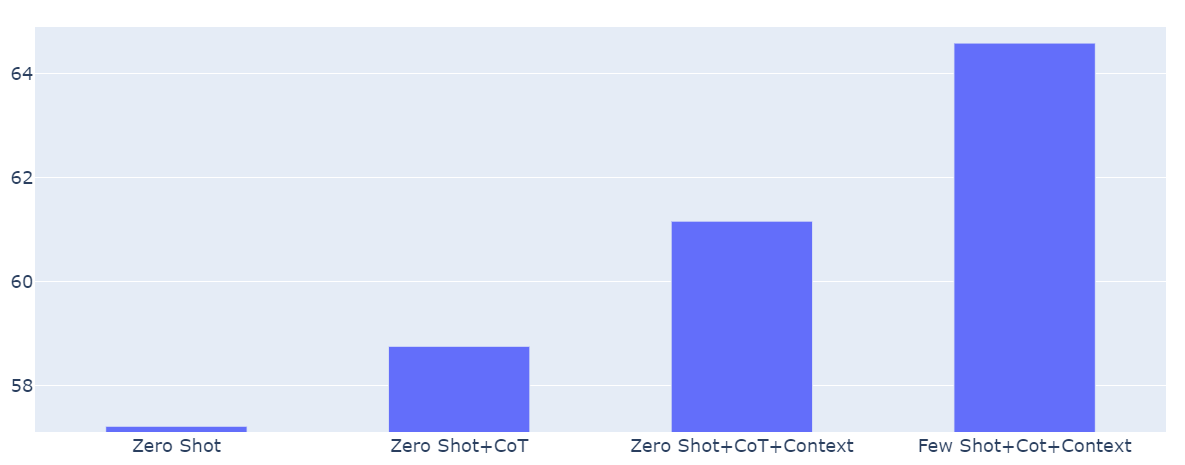
\includegraphics[width=0.9\linewidth]{images/prompt-result.png}}
	\caption{مقدار
		\lr{F1-Score}
		هر یک از تکنیک‌های پیش‌پردازش داده}
	\label{prompt-result-chart}
\end{figure}


 
در ادامه برای بررسی اثربخشی پیش‌پردازش متن ورودی بر خروجی مدل زبانی بزرگ، آزمایش‌ها برای پرامپت
\lr{Zero Shot + CoT + Context}
تکرار شد. در این آزمایش‌ها سه روش متفاوت برای پیش‌پردازش داده‌ها را که در فصل قبل عملکرد بهتری از خود نشان دادند مورد بررسی قرار گرفت. نتایج به دست آمده در جدول~
\ref{prompt-data-cleaning-impact}
گزارش شده است. در نمودار
\ref{prompt-data-cleaning-impact-chart}
نتایج به دست آمده به صورت شهودی قابل مقایسه است. همان‌طور که نتایج نشان می‌دهد، با تغییر روش پیش‌پردازش داده‌ها تغییر معنی‌داری در نتایج به دست آمده به وجود نمی‌آید. 
\begin{table}[h!]
	\centering
	\small
	\caption{\label{prompt-data-cleaning-impact}تاثیر پیش‌پردازش داده‌ها در نتایج به دست آمده}
	\vspace{0.2cm}
	\begin{tabular}{c  |c }
	\hline
	پیش‌پردازش & $F1-Score$\\
	\hline
	
	%Data prompt precirion Recall F1 accuract
	
	%Run8 Real Data P6 0.6233 0.6122 0.6116	0.6197	
	بدون پیش‌پردازش&  $61.16$
	%& $61.97$
	\\
	
	%Run12 Remove url P6 0.6268	0.6090	0.6157	0.6114
	حذف آدرس اینترنتی&  $61.57$\\
	%Run13 Remove username P6 0.6283 0.6216	0.6119	0.6236
حدف نام کاربری&  $61.19$\\
	%Run14	Remove url+username P6	0.6261	0.6102	0.6165	0.6069	
	حذف همزمان آدرس اینترنتی و نام کاربری&  $61.65$\\
	\hline
	\hline
\end{tabular}
\end{table}

\begin{figure}[H]
	\center{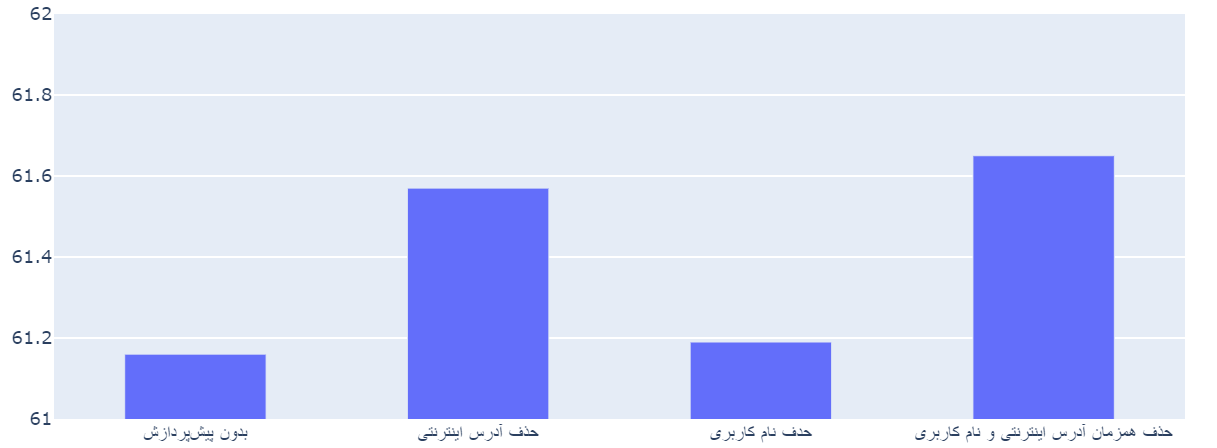
\includegraphics[width=0.9\linewidth]{images/prompt-data-cleaning-impact-chart.png}}
	\caption{مقدار
		\lr{F1-Score}
		هر یک از تکنیک‌های پیش‌پردازش داده}
	\label{prompt-data-cleaning-impact-chart}
\end{figure}


\subsection{مزایا و معایب روش پیشنهادی}
از جمله مزایای روش پیشنهادی، پیش‌بینی خروجی بدون نیاز به داده‌ آموزشی یا با وجود داده‌های آموزشی کم می‌باشد. بر خلاف روش فصل پنجم، استفاده از پرامپت 
\lr{Domain Specific}
نیست و بر دامنه‌های مختلف می‌توان نتایج قابل قبولی دریافت کرد.

از طرفی نیاز به منابع محاسباتی 
\lr{GPU}
با رم بالا از جمله معایب این روش می‌باشد. همچنین به دلیل اینکه پرامپت توسط نیروی انسانی طراحی می‌شود، ممکن است پرامپت کاملا بهینه‌ای طراحی نشده باشد. علاوه امکان 
\lr{fine-tuning}
پرامپت‌های پیشنهادی برای مدل با توجه به منابع محاسباتی محدود، مقدور نمی‌باشد.
\subsection{نحوه پیاده‌سازی و اجرا آزمایش‌ها}
پیاده‌سازی پروژه در 
\href{https://github.com/ghazaleh-mahmoodi/Climate_Activism_Stance_Detection}{اینجا}
\LTRfootnote{\href{https://github.com/ghazaleh-mahmoodi/Climate_Activism_Stance_Detection}{https://github.com/ghazaleh-mahmoodi/Climate\_Activism\_Stance\_Detection}}
قابل مشاهده می‌باشد که با زبان پایتون و فریم‌ورک پایتورچ انجام شده است. برای تعامل با مدل زبانی بزرگ از 
\lr{guidance}\LTRfootnote{\href{https://github.com/guidance-ai/guidance}{https://github.com/guidance-ai/guidance}}
استفاده شده است. هر بار پیشبینی برای کل داده‌های ارزیابی با توجه به نوع پرامپت حدود 40 الی 160 دقیقه زمان می‌برد. زمان تقریبی تولید خروجی برای یک ورودی حدود 4 الی 15 ثانیه می‌باشد.
\newline
برای اجرا از سخت‌افزار
\lr{GPU.1080Ti.xlarge}
با رم 
\lr{31.3GB}
استفاده شد. دستور 
\lr{nvidia-smi}
میزان استفاده از 
\lr{GPU}
را نمایش می‌دهد. خروجی این دستور در هنگام اجرا آزمایشات به صورت شکل 
\ref{nvidia-smi-prompt} شد.
\begin{figure}[H]		  		    			  	 \center{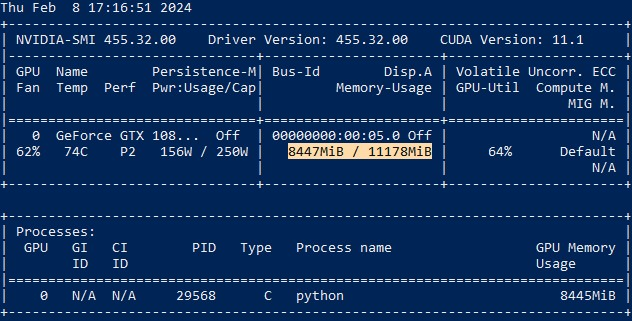
\includegraphics[width=0.8\linewidth]{images/nvidia-smi-prompt.jpg}}
	\caption{میزان مصرف \lr{GPU}در زمان اجرا آزمایش‌های مدل‌های زبانی بزرگ}
	\label{nvidia-smi-prompt}
\end{figure}

%\section{جمع‌بندی}


